\documentclass[10pt]{beamer}

\usetheme[progressbar=frametitle]{metropolis}
\usepackage{appendixnumberbeamer}

\usepackage{booktabs}
\usepackage[scale=2]{ccicons}

\usepackage{pgfplots}
\usepgfplotslibrary{dateplot}

\usepackage{xspace}
\newcommand{\themename}{\textbf{\textsc{metropolis}}\xspace}

\usepackage{caption}
%\usepackage{gensymb}
\usepackage{ulem}
\usepackage{subcaption}
\usepackage[french]{babel}
\usepackage{csquotes}
\usepackage[backend=biber,style=authoryear,citestyle=authoryear]{biblatex}

\DeclareCaptionLabelFormat{underlcap}{\uline{#1 #2}}
\DeclareCaptionLabelSeparator{underlcap}{~}
\DeclareCaptionTextFormat{underlcap}{\expandafter\uline\expandafter{\expandafter#1}}

\captionsetup[figure]{%
   labelformat=underlcap,labelseparator=underlcap,textformat=underlcap}
   
\newcommand\Wider[2][3em]{%
\makebox[\linewidth][c]{%
  \begin{minipage}{\dimexpr\textwidth+#1\relax}
  \raggedright#2
  \end{minipage}%
  }%
}

\makeatletter
\setlength{\metropolis@progressinheadfoot@linewidth}{1.7pt}
\setlength{\metropolis@titleseparator@linewidth}{1.7pt}
\setlength{\metropolis@progressonsectionpage@linewidth}{1.7pt}

\definecolor{alizarin}{rgb}{0.1, 0.26, 0.82}
\definecolor{bazaar}{rgb}{0.63, 0.63, 0.8}

\setbeamercolor{progress bar}{fg=alizarin,bg=bazaar}

\AtBeginSection[]{
  \begin{frame}
  \vfill
  \centering
  \begin{beamercolorbox}[sep=8pt,center,shadow=true,rounded=true]{title}
    \usebeamerfont{title}\insertsectionhead\par%
  \end{beamercolorbox}
  \vfill
  \end{frame}
}

\addbibresource{/Applications/ZoteroBibs/Library.bib}

\title{Prédire l'humidité troposphérique en fonction de l'organisation de la convection et de la circulation de grande échelle}
\subtitle{Félix Langot}
\date{\today}
\author{\textit{LMD - UVSQ/Paris-Saclay}}
\institute{}
% \titlegraphic{\vfill
\includegraphics[height=1.5cm]{Figures/logo.png}}
\begin{document}

\maketitle

\section*{Introduction}
\begin{frame}{\secname}

    \begin{itemize}
        \setlength{\itemsep}{7pt}
        \item \textbf{But du stage:} développer un modèle théorique simple pour quantifier l'effet de l'organisation de la convection et de la circulation de grande échelle sur l'humidité de la troposphère 
        \item Utilisation de simulations CRMs $\rightarrow$ vérifier les hypothèses du modèle + évaluer son réalisme. 
        \item Différentes distributions de l'humidité relative (RH) dans la troposphère, dues à: \\
        $\rightarrow$ l'agrégation de la convection: fait baisser la RH  \\
        $\rightarrow$ l'ascendance: humidifie la troposphère \\
        \autocite{Tobin2012}
    \end{itemize}

\end{frame}

\begin{frame}{\secname}
    \begin{itemize}
        \item \textbf{Simulation en équilibre radiatif-convectif (RCE) sur Cloud-Resolving  Model  (CRM):}
    \end{itemize}
    \begin{figure}[hbtp]
        \centering
        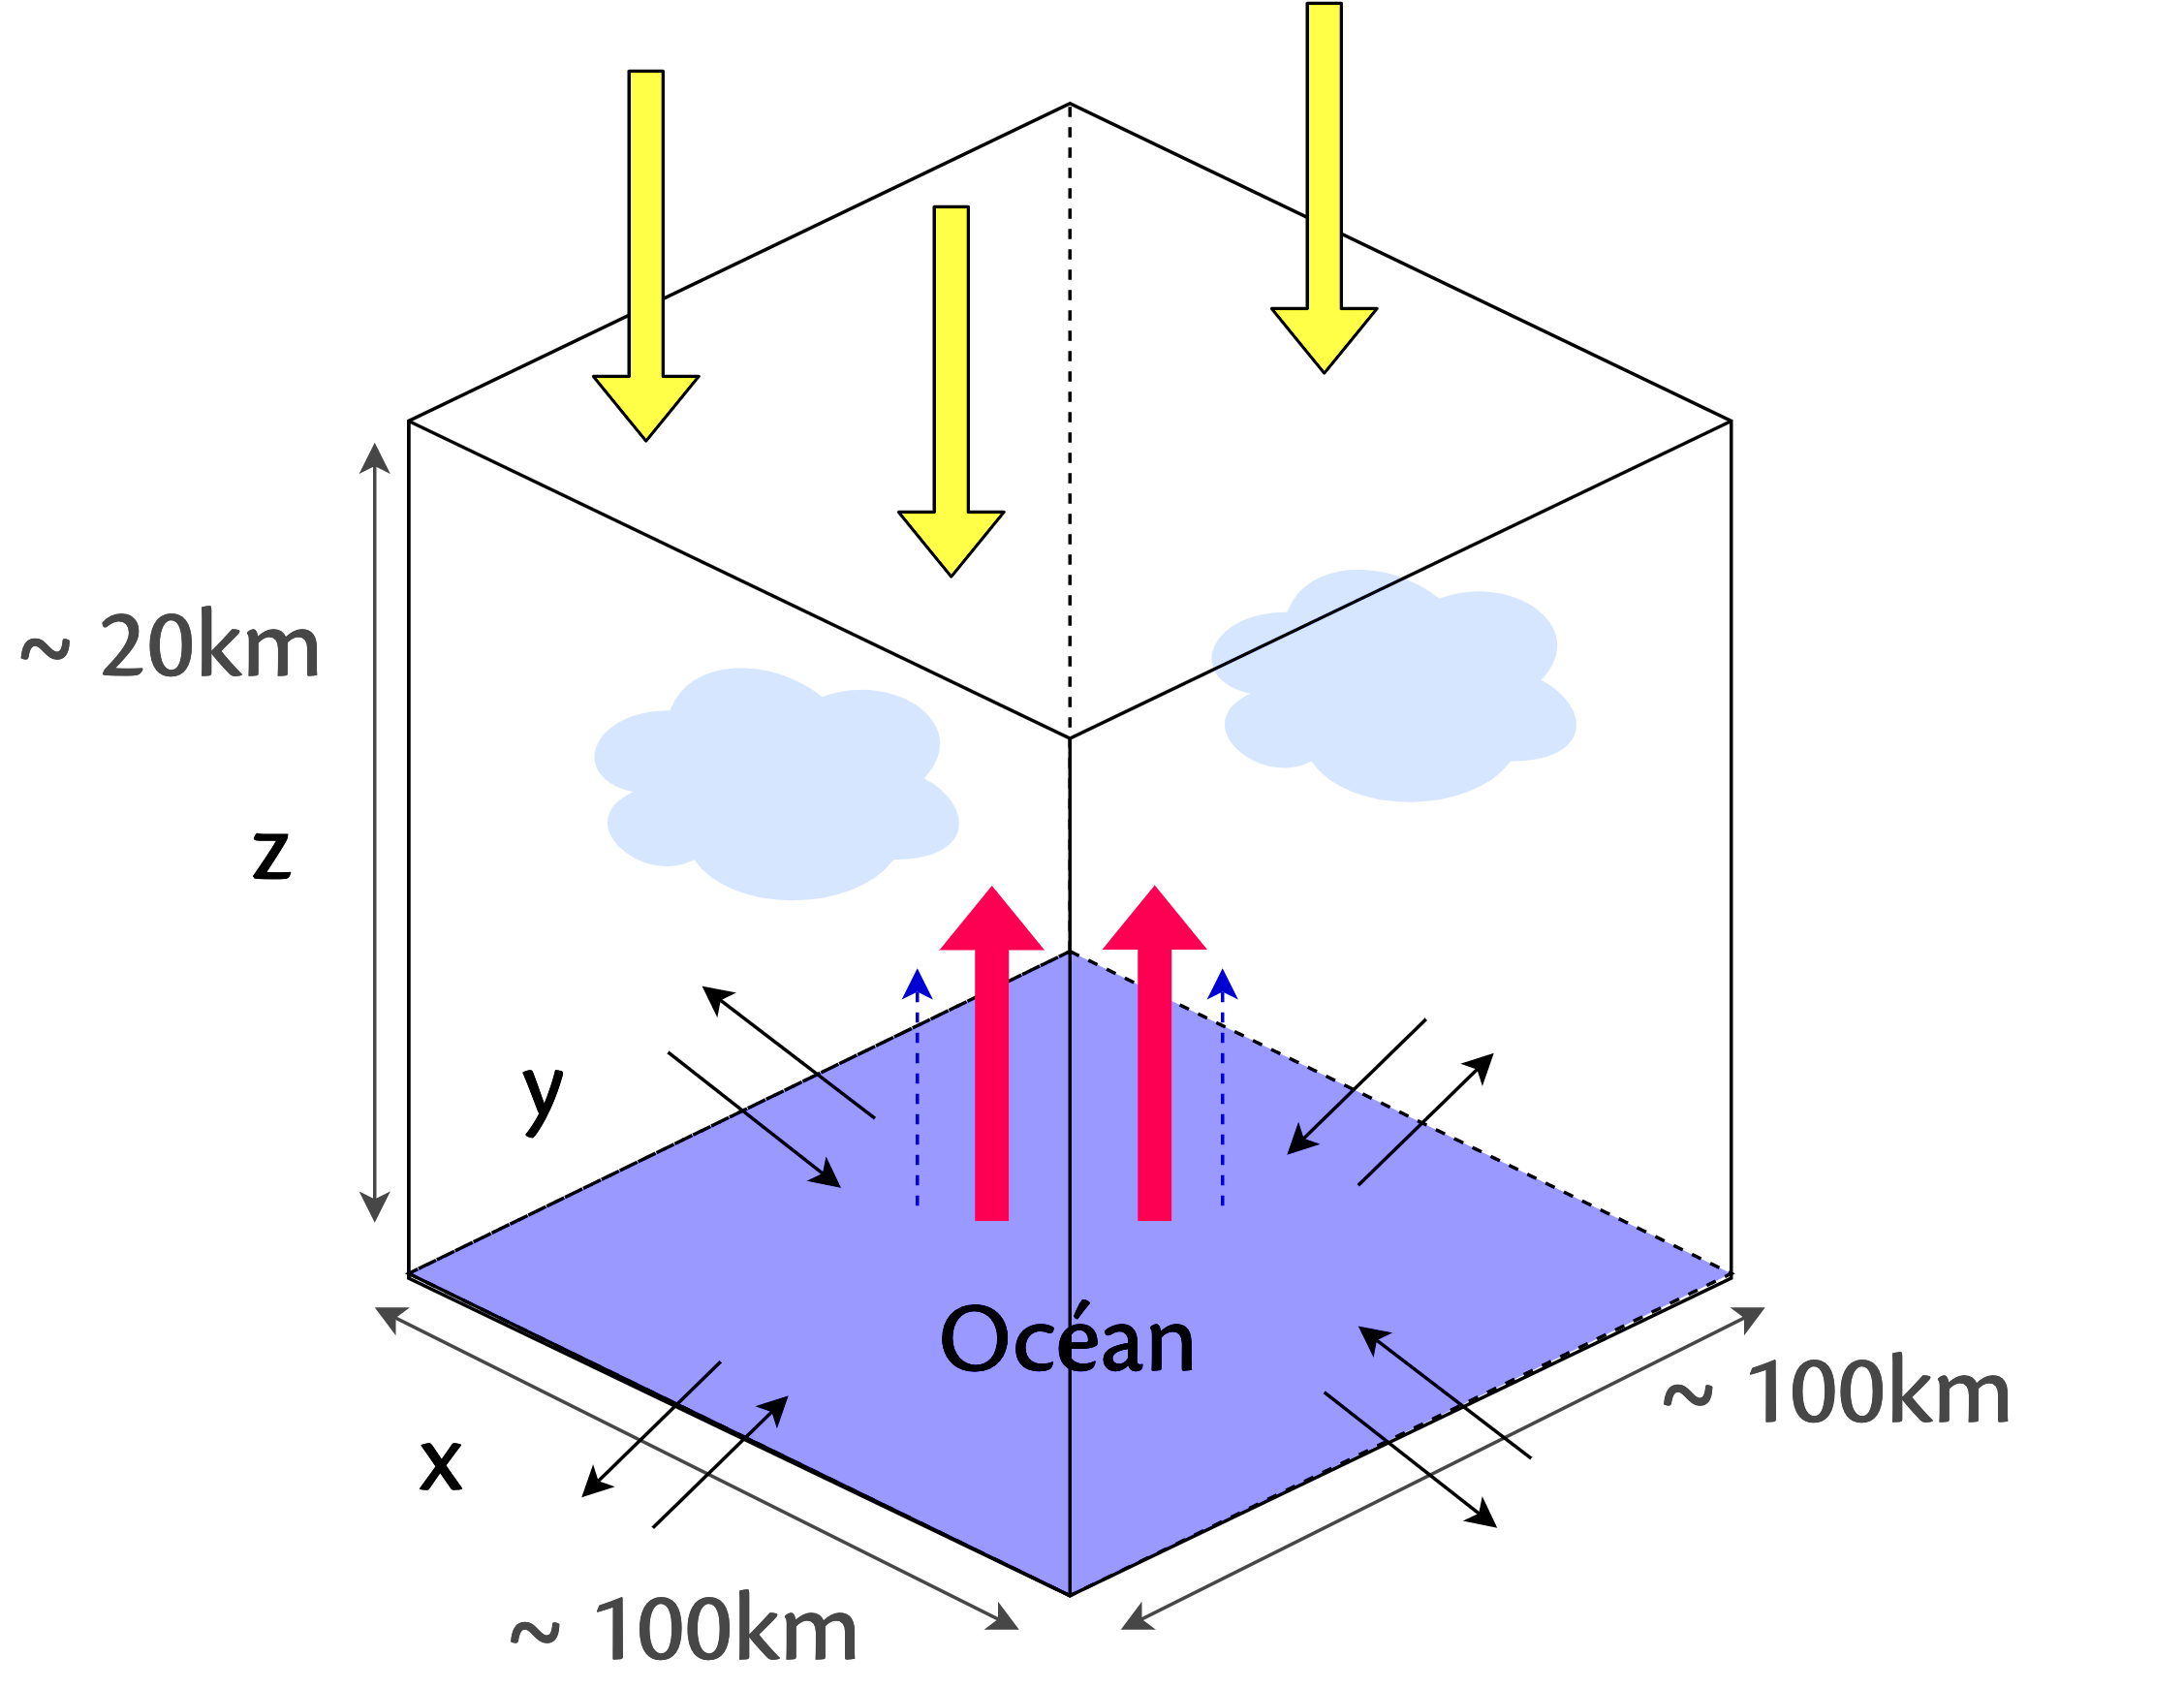
\includegraphics[width=6.2cm]{Figures/CRM.png}    
    \end{figure}
\end{frame}

\begin{frame}{\secname}
\Wider{
    \begin{itemize}
        \setlength{\itemsep}{5pt}
        \item \textbf{Pourquoi et comment représenter la circulation de grande-échelle:} 
        \begin{itemize}
            \setlength{\itemsep}{5pt}
            \item Impacte l'humidité de l'atmosphère par advection mais aussi l'organisation de la convection \autocite{dufauxRapportStageLicence2021}, qui à son tour modifie la RH. 
            \item Représenter l’ascendance de grande échelle $\rightarrow$ ajout d'un terme d’advection verticale d’humidité et de température.
        \end{itemize}
    \end{itemize}
}
\end{frame}

\begin{frame}
    \begin{itemize}
        \item \textbf{Obtention de différents types d'organisation:} On ajoute au RCE un forçage différent en fonction du type d'organisation que l'on veut favoriser
    \end{itemize}
    \begin{figure}[hbtp]
        \centering
        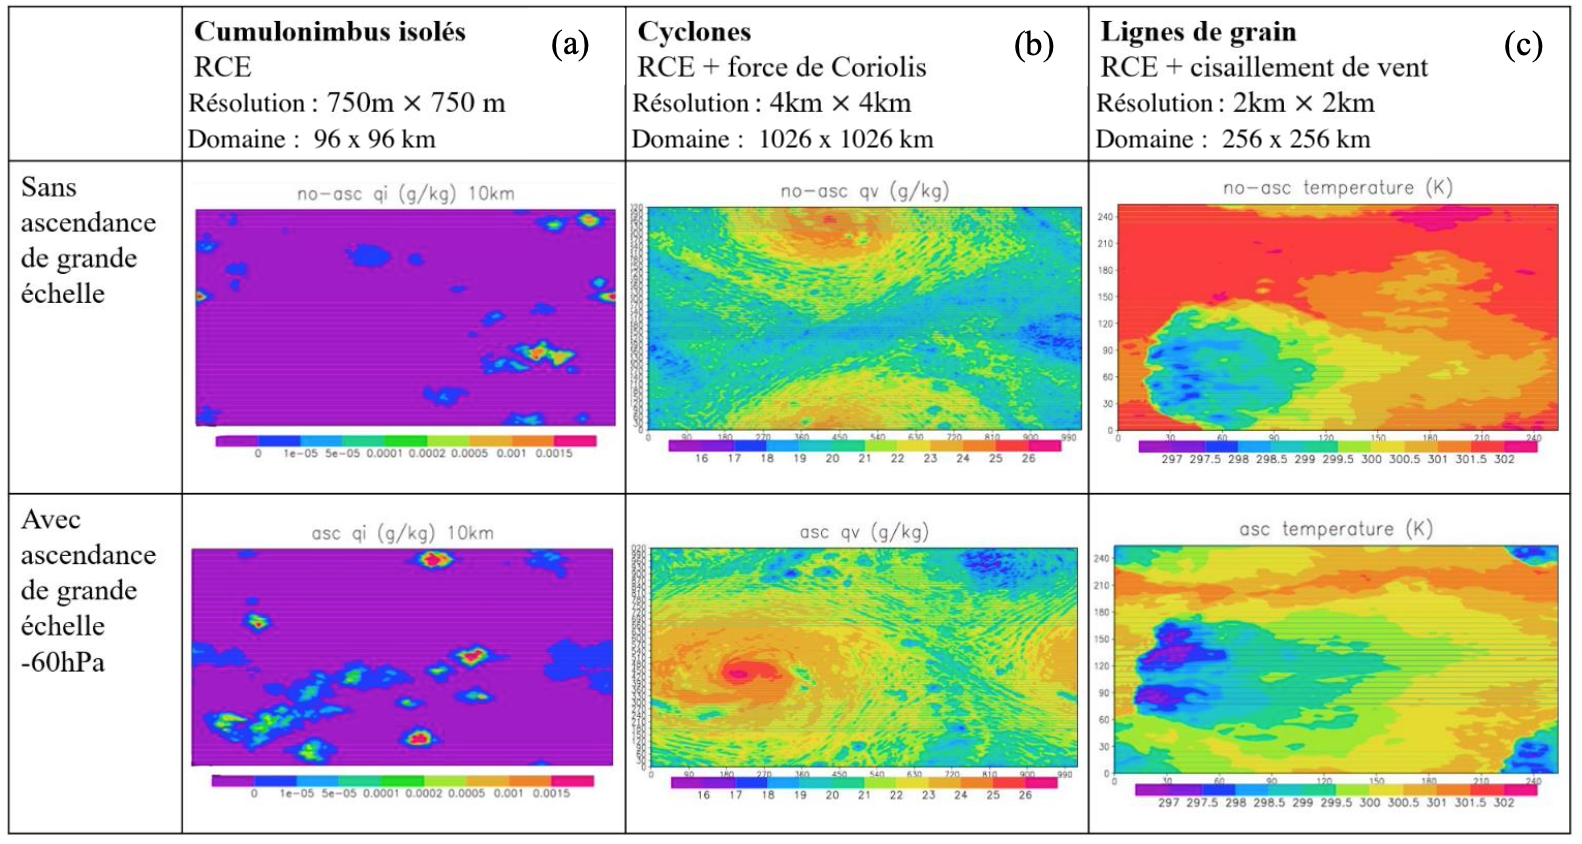
\includegraphics[width=11cm]{Figures/DufauxTable.png}
    \end{figure}
\end{frame}

\begin{frame}{\secname}
\begin{columns}
    \column{0.4\textwidth}
    \begin{itemize}
        \item Effets vérifiés par le CRM SAM, avec lequel on calcule l'humidité
        $$
        RH_{actual} = \left.\frac{q_v}{q_{sat}}\right|_{z_{parcel}=5km}
        $$
    \end{itemize}
    \column{0.6\textwidth}
    \begin{figure}
        \centering
        \includegraphics[width=7cm]{../Codes/Figs/RHaProbsSuperposition.png}
        \label{RHactual0}
    \end{figure}
\end{columns}
\end{frame}

\section*{Comment prédire les distributions de \textit{RH}?}
\begin{frame}{\secname}
     \begin{itemize}
         \item Pour prédire les distributions de RH, on utilise le modèle d'advection-condensation \autocite{pierrehumbertRelativeHumidityAtmosphere2007,Vallis2017}
     \end{itemize}
     \vspace{-1cm}
     \begin{columns}
         \column{0.55\textwidth}
         \begin{itemize}
            \item Ascendance + Organisation \\ $\rightarrow$ probabilité d'humidification
        \end{itemize}
         \column{0.6\textwidth}
         \begin{figure}[hbtp]
            \centering
            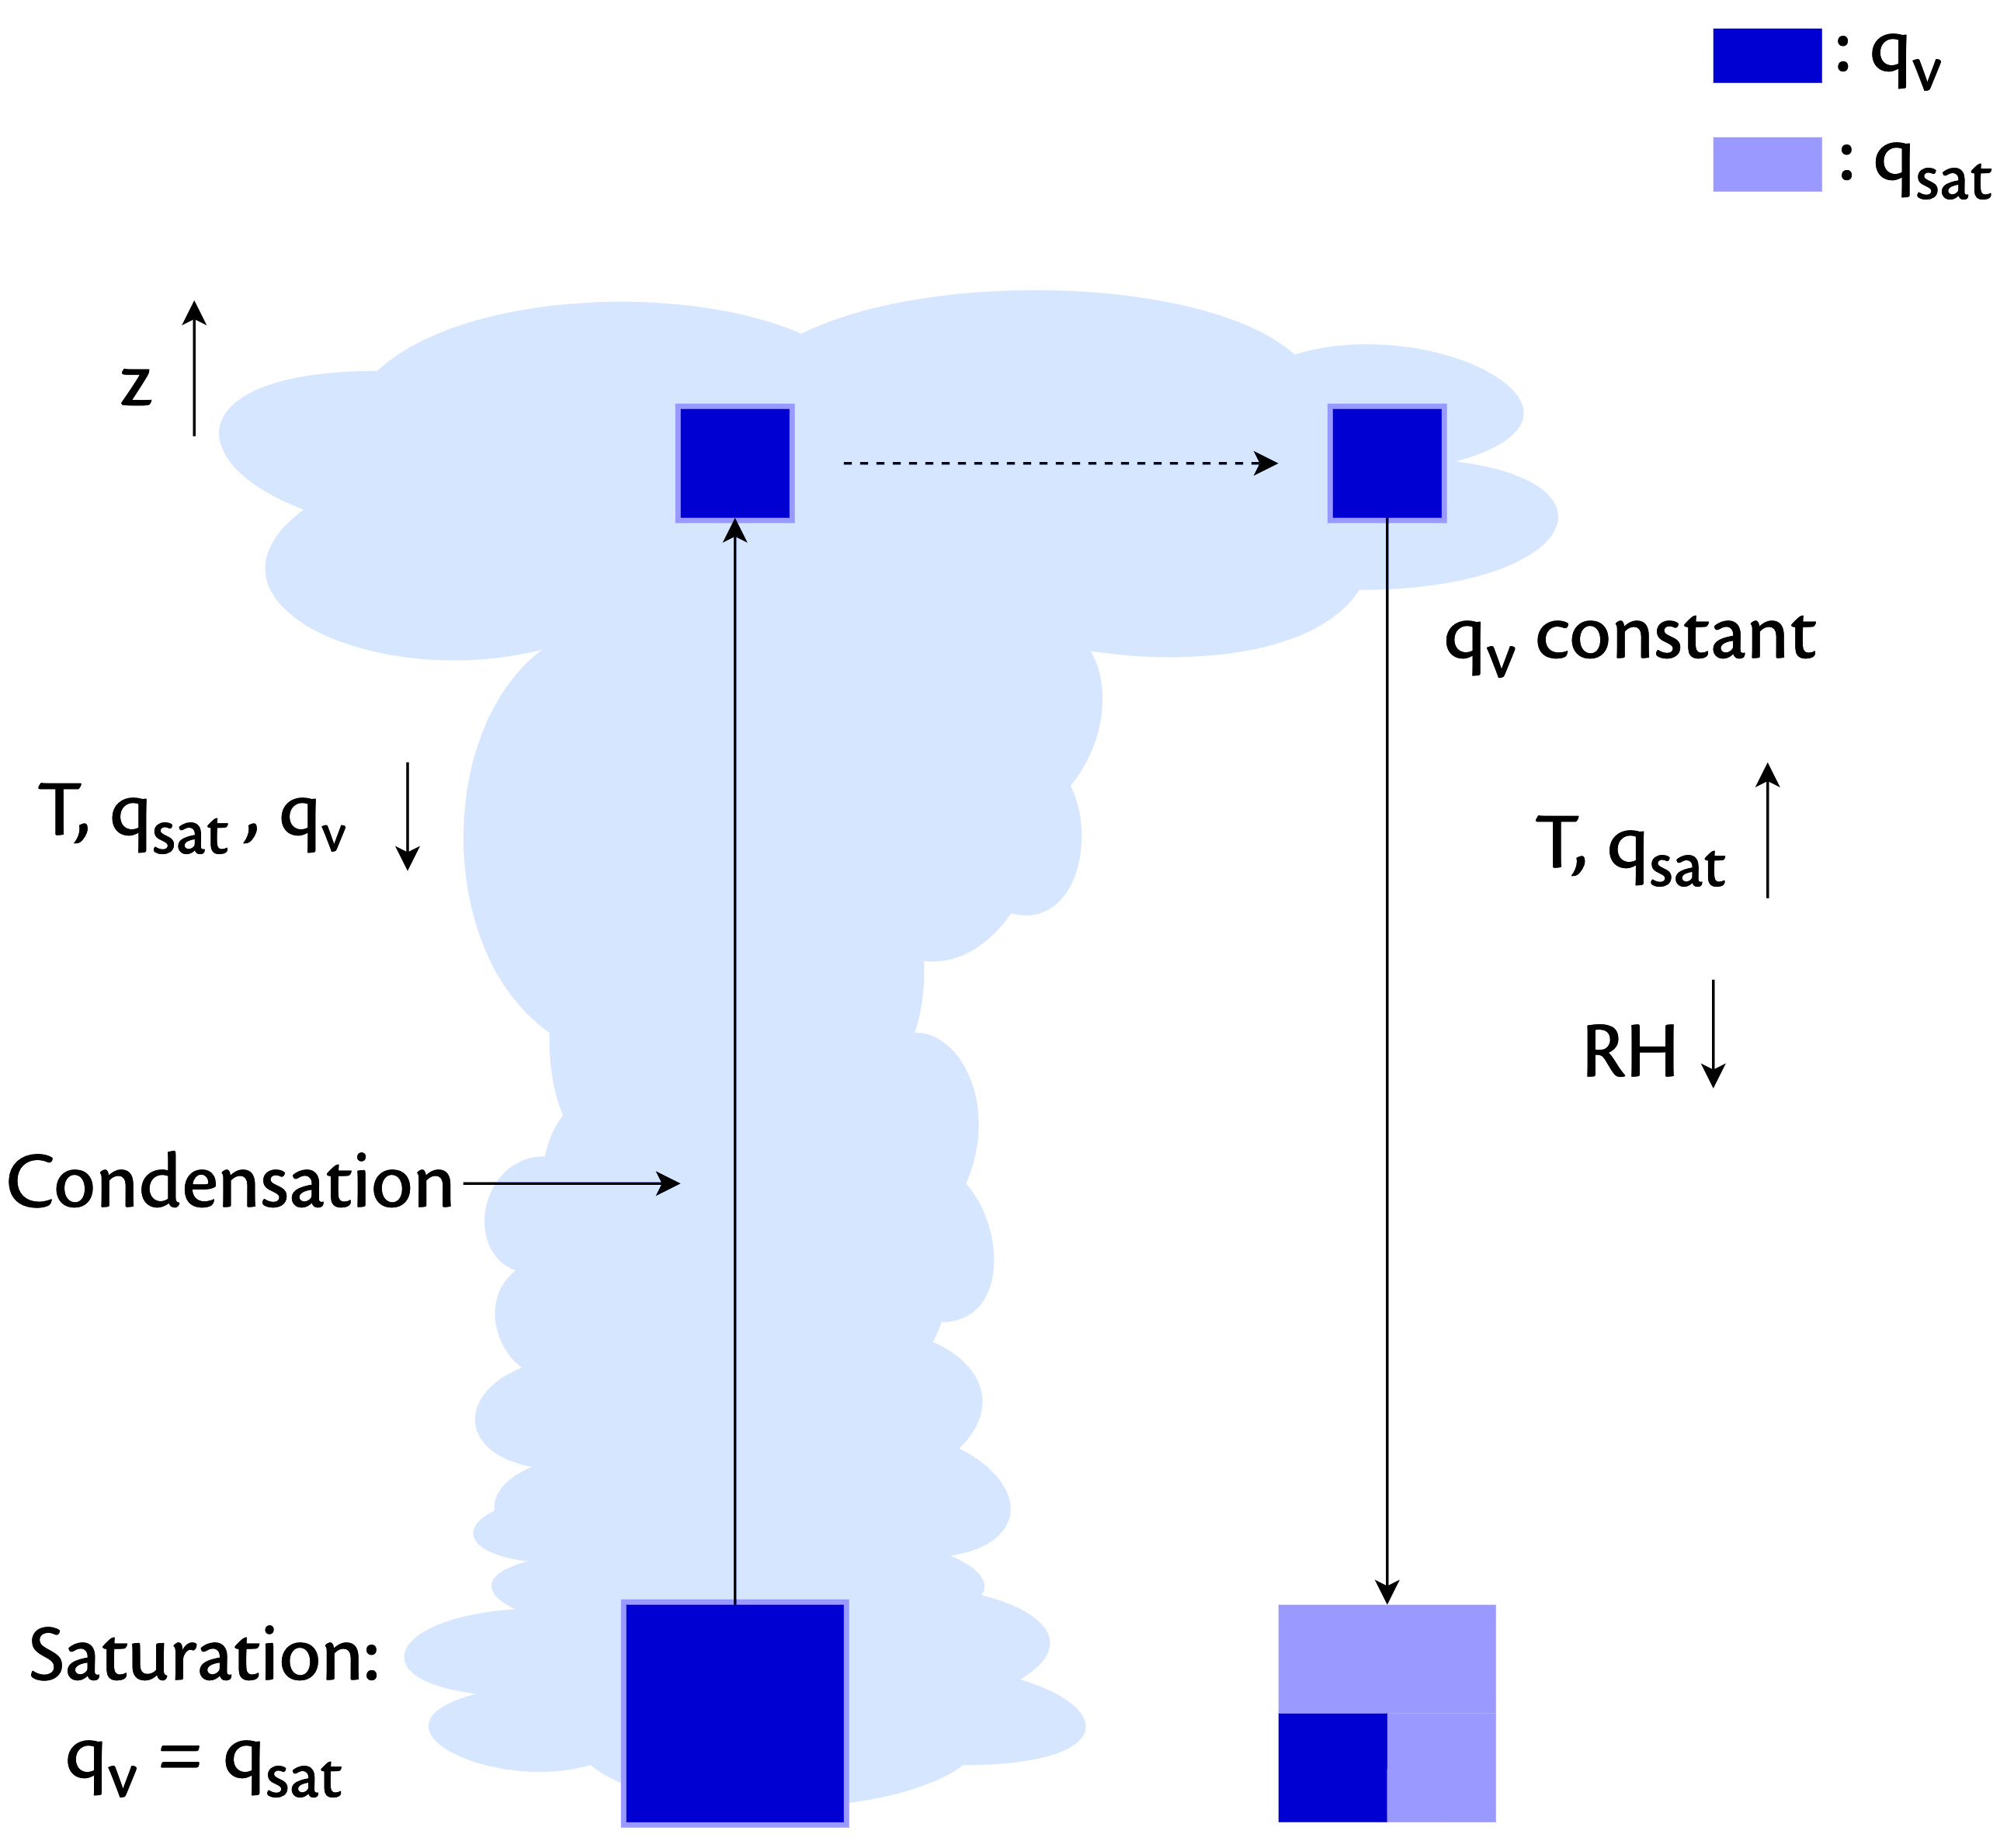
\includegraphics[width=6.6cm]{Figures/advec-condens.png}
        \end{figure}
     \end{columns}
\end{frame}

\section*{Altitude de dernière saturation - Approche statique}
\begin{frame}{\secname}
    \begin{itemize}
        \setlength{\itemsep}{4pt}
        \item \textbf{Hypothèse statique:} L'altitude de dernière saturation d'une parcelle troposphérique correspond à l'altitude du nuage le plus proche au-dessus de la parcelle.
        \item SAM: $q_c + q_i > 10^{-6}$ alors le point de grille est dans un nuage \autocite{Risi2021}
    \end{itemize}
    \begin{figure}[hbtp]
        \centering
        \includegraphics[width=6cm]{../Codes/Figs/lastsaturationlight.png}
    \end{figure}
\end{frame}

\begin{frame}{\secname}
    On peut donc mesurer l'altitude du nuage le plus proche de chaque point de grille à chaque pas de temps des simulations
    \begin{figure}[hbtp]
        \centering
        \includegraphics[width=10cm]{../Codes/Figs/3Dclouds.png}
    \end{figure}
\end{frame}

\begin{frame}{\secname}
    L'humidité relative prédite RH$_p$ peut ensuite être calculée en fonction de $q_{sat}$ seulement:
    $$
    RH_p = \frac{q_{sat}(z_{clouds})}{q_{sat}(z_{parcel})}
    $$
    où $z_{clouds}$ est l'altitude des nuages les plus proches de la troposphère au-dessus des points de grille à $z_{parcel} = 5km$, l'altitude choisie dans la troposphère
\end{frame}

\begin{frame}{\secname}
    On peut comparer la distribution obtenue avec cette méthode à la distribution réelle de la RH
    \Wider{
        \begin{figure}[hbtp]
            \centering
            \includegraphics[width=12cm]{../Codes/Figs/RhvsRHp.png}
        \end{figure}
    $\rightarrow$ La RH ne peut pas être prédite par un modèle statique \\ 
    $\rightarrow$ Intermittence des nuages + mouvement de la parcelle importants.
        }
\end{frame}

\section*{Altitude de dernière saturation - Approche dynamique}

\begin{frame}{\secname}
\Wider{
\textbf{Approche dynamique:} On considère le mouvement vertical d'une parcelle au-dessus de la troposphère. L'altitude de dernière saturation d'une parcelle à 5km au pas de temps $t$ est l'altitude à laquelle elle a rencontré un nuage pour la dernière fois le long de sa trajectoire à $t-\Delta T$. 

    \begin{figure}[hbtp]
        \centering
        \includegraphics[width=7cm]{../Codes/Figs/lastsaturationsubsidencelight.png}
    \end{figure}
}
\end{frame}

\begin{frame}{\secname}
    \begin{itemize}
        \item SAM $\rightarrow w \rightarrow w_{env}$     
        \item Simulations avec ascendance: $w_{tot} = w_{env} + w_{LS}$, où $w_{LS}$ est l'ascendance imposée.
    \end{itemize} 
    \begin{figure}[hbtp]
        \centering
        \includegraphics[width=7cm]{../Codes/Figs/wtotz.png}
    \end{figure}
\end{frame}

\begin{frame}{\secname}
    \begin{itemize}
        \item On trace la trajectoire de la parcelle, gouvernée par $w_{tot}$.
    \end{itemize}
    \begin{figure}[hbtp]
        \centering
        \includegraphics[width=7.5cm]{../Codes/Figs2/ztraj.png}
    \end{figure}
\end{frame}

\begin{frame}{\secname}
    En utilisant les mêmes conditions pour détecter les nuages, on obtient les altitudes de dernières saturations suivantes:
    \begin{figure}[hbtp]
        \centering
        \includegraphics[width=10cm]{../Codes/Figs2/zclouds_traj.png}
    \end{figure}
\end{frame}

\section*{Résultats}

\begin{frame}{\secname}
    Et l'humidité correspondante avec 
    $$
    RH_p = \frac{q_{sat}(z_{clouds})}{q_{sat}(z_{parcel})}
    $$
    \Wider{
    \begin{figure}[hbtp]
        \centering
        \includegraphics[width=12cm]{../Codes/Figs2/zcloudsvsRHp.png}
    \end{figure}
    }
\end{frame}

\begin{frame}{\secname}
    On compare les distributions obtenues avec les différents calculs d'humidité
    \Wider{
    \begin{figure}[hbtp]
        \centering
        \includegraphics[width=9cm]{../Codes/Figs2/RhvsRHovsRHp.png}
    \end{figure}
    }
\end{frame}

\section*{Influence du pas de temps}

\begin{frame}{\secname}

    \begin{figure}[hbtp]
        \centering
        \includegraphics[width=10cm]{../Codes/Figs2/RHps.png}
    \end{figure}
    
\end{frame}

\begin{frame}[allowframebreaks]{Bibliographie}
    \printbibliography
\end{frame}


\end{document}
